\documentclass[3p]{elsarticle}

\usepackage{lineno,hyperref}
\modulolinenumbers[5]

\journal{Journal of \LaTeX\ Templates}

%%%%%%%%%%%%%%%%%%%%%%%
%% Elsevier bibliography styles
%%%%%%%%%%%%%%%%%%%%%%%
%% To change the style, put a % in front of the second line of the current style and
%% remove the % from the second line of the style you would like to use.
%%%%%%%%%%%%%%%%%%%%%%%

%% Numbered
%\bibliographystyle{model1-num-names}

%% Numbered without titles
%\bibliographystyle{model1a-num-names}

%% Harvard
%\bibliographystyle{model2-names.bst}\biboptions{authoryear}

%% Vancouver numbered
%\usepackage{numcompress}\bibliographystyle{model3-num-names}

%% Vancouver name/year
\usepackage{numcompress}\bibliographystyle{model4-names}\biboptions{authoryear}

%% APA style
%\bibliographystyle{model5-names}\biboptions{authoryear}

%% AMA style
%\usepackage{numcompress}\bibliographystyle{model6-num-names}

%% `Elsevier LaTeX' style
\bibliographystyle{elsarticle-num}
%%%%%%%%%%%%%%%%%%%%%%%

\graphicspath{{./figure/}}




\usepackage{lineno,hyperref}

\usepackage{galois} % composition function \comp
\usepackage{bm}
\usepackage{amsmath}
\usepackage{amssymb}
\usepackage{mathrsfs}
\usepackage{amsthm}
\usepackage{natbib}
\usepackage{graphicx}
\usepackage{color}
\usepackage{booktabs}
\usepackage[page,title]{appendix}
%\renewcommand\appendixname{haha}
\usepackage{enumerate}
\usepackage{changepage}
\usepackage{datetime}
\newdate{date}{9}{1}{2017}

%%%%%%%%%% page setup %%%%%%%%%%
\textheight 8.5 in
\textwidth 6.5 in
\topmargin -0.5 in
\oddsidemargin -0.1 in
%%%%%%%%%%%%%%  Notations %%%%%%%%%%
\DeclareMathOperator{\mytr}{tr}
\DeclareMathOperator{\mydiag}{diag}
\DeclareMathOperator{\myrank}{Rank}
\DeclareMathOperator{\myP}{P}
\DeclareMathOperator{\myE}{E}
\DeclareMathOperator{\myVar}{Var}
\DeclareMathOperator*{\argmax}{arg\,max}
\DeclareMathOperator*{\argmin}{arg\,min}


\newcommand{\Ba}{\mathbf{a}}    \newcommand{\Bb}{\mathbf{b}}    \newcommand{\Bc}{\mathbf{c}}    \newcommand{\Bd}{\mathbf{d}}    \newcommand{\Be}{\mathbf{e}}    \newcommand{\Bf}{\mathbf{f}}    \newcommand{\Bg}{\mathbf{g}}    \newcommand{\Bh}{\mathbf{h}}    \newcommand{\Bi}{\mathbf{i}}    \newcommand{\Bj}{\mathbf{j}}    \newcommand{\Bk}{\mathbf{k}}    \newcommand{\Bl}{\mathbf{l}}
\newcommand{\Bm}{\mathbf{m}}    \newcommand{\Bn}{\mathbf{n}}    \newcommand{\Bo}{\mathbf{o}}    \newcommand{\Bp}{\mathbf{p}}    \newcommand{\Bq}{\mathbf{q}}    \newcommand{\Br}{\mathbf{r}}    \newcommand{\Bs}{\mathbf{s}}    \newcommand{\Bt}{\mathbf{t}}    \newcommand{\Bu}{\mathbf{u}}    \newcommand{\Bv}{\mathbf{v}}    \newcommand{\Bw}{\mathbf{w}}    \newcommand{\Bx}{\mathbf{x}}
\newcommand{\By}{\mathbf{y}}    \newcommand{\Bz}{\mathbf{z}}    
\newcommand{\BA}{\mathbf{A}}    \newcommand{\BB}{\mathbf{B}}    \newcommand{\BC}{\mathbf{C}}    \newcommand{\BD}{\mathbf{D}}    \newcommand{\BE}{\mathbf{E}}    \newcommand{\BF}{\mathbf{F}}    \newcommand{\BG}{\mathbf{G}}    \newcommand{\BH}{\mathbf{H}}    \newcommand{\BI}{\mathbf{I}}    \newcommand{\BJ}{\mathbf{J}}    \newcommand{\BK}{\mathbf{K}}    \newcommand{\BL}{\mathbf{L}}
\newcommand{\BM}{\mathbf{M}}    \newcommand{\BN}{\mathbf{N}}    \newcommand{\BO}{\mathbf{O}}    \newcommand{\BP}{\mathbf{P}}    \newcommand{\BQ}{\mathbf{Q}}    \newcommand{\BR}{\mathbf{R}}    \newcommand{\BS}{\mathbf{S}}    \newcommand{\BT}{\mathbf{T}}    \newcommand{\BU}{\mathbf{U}}    \newcommand{\BV}{\mathbf{V}}    \newcommand{\BW}{\mathbf{W}}    \newcommand{\BX}{\mathbf{X}}
\newcommand{\BY}{\mathbf{Y}}    \newcommand{\BZ}{\mathbf{Z}}    

\newcommand{\bfsym}[1]{\ensuremath{\boldsymbol{#1}}}

\def\balpha{\bfsym \alpha}
\def\bbeta{\bfsym \beta}
\def\bgamma{\bfsym \gamma}             \def\bGamma{\bfsym \Gamma}
\def\bdelta{\bfsym {\delta}}           \def\bDelta {\bfsym {\Delta}}
\def\bfeta{\bfsym {\eta}}              \def\bfEta {\bfsym {\Eta}}
\def\bmu{\bfsym {\mu}}                 \def\bMu {\bfsym {\Mu}}
\def\bnu{\bfsym {\nu}}
\def\btheta{\bfsym {\theta}}           \def\bTheta {\bfsym {\Theta}}
\def\beps{\bfsym \varepsilon}          \def\bepsilon{\bfsym \varepsilon}
\def\bsigma{\bfsym \sigma}             \def\bSigma{\bfsym \Sigma}
\def\blambda {\bfsym {\lambda}}        \def\bLambda {\bfsym {\Lambda}}
\def\bomega {\bfsym {\omega}}          \def\bOmega {\bfsym {\Omega}}
\def\brho   {\bfsym {\rho}}
\def\btau{\bfsym {\tau}}
\def\bxi{\bfsym {\xi}}
\def\bzeta{\bfsym {\zeta}}
% May add more in future.
%%%%%%%%%%%%%%%%%%%%%%%%%%%%%%%%%%%%



\theoremstyle{plain}
\newtheorem{theorem}{\quad\quad Theorem}
\newtheorem{proposition}{\quad\quad Proposition}
\newtheorem{corollary}{\quad\quad Corollary}
\newtheorem{lemma}{\quad\quad Lemma}
\newtheorem{example}{Example}
\newtheorem{assumption}{\quad\quad Assumption}
\newtheorem{condition}{\quad\quad Condition}

\theoremstyle{definition}
\newtheorem{remark}{\quad\quad Remark}
\theoremstyle{remark}

\begin{document}

\begin{frontmatter}

\title{Integrated likelihood ratio test\tnoteref{mytitlenote}}
\tnotetext[mytitlenote]{Fully documented templates are available in the elsarticle package on \href{http://www.ctan.org/tex-archive/macros/latex/contrib/elsarticle}{CTAN}.}

%% Group authors per affiliation:
\author{author \fnref{myfootnote}}
\address{Radarweg 29, Amsterdam}
\fntext[myfootnote]{Since 1880.}

%% or include affiliations in footnotes:
\author[mymainaddress,mysecondaryaddress]{Elsevier Inc}
\ead[url]{www.elsevier.com}

\author[mysecondaryaddress]{Global Customer Service\corref{mycorrespondingauthor}}
\cortext[mycorrespondingauthor]{Corresponding author}
\ead{support@elsevier.com}

\address[mymainaddress]{1600 John F Kennedy Boulevard, Philadelphia}
\address[mysecondaryaddress]{360 Park Avenue South, New York}

\begin{abstract}

    Likelihood ratio test (LRT) is the most widely used test procedure. However, it has some weaknesses. Likelihood is unbounded for some important models. Even when the likelihood is bounded, the maximum may be not easy to obtain if it is not convex in parameters. We propose a new test procedure called integrated likelihood ratio test (ILRT) which can overcome the above difficulties. Posterior Bayes factor is a special case of ILRT\@. We proof the Wilks phenomenon of ILRT and give the asymptotic local power.
\end{abstract}

\begin{keyword}
%\texttt{elsarticle.cls} \sep \LaTeX \sep Elsevier \sep template
%\MSC[2010] 00-01\sep  99-00
\end{keyword}

\end{frontmatter}

%\linenumbers

\section{Introduction}
Suppose that we have $n$ observations $\BX^{(n)}=(X_1,\ldots,X_n)$ which are independent identically distributed (i.i.d.) random variables with values in some space space $(\mathcal{X};\mathscr{A})$.
Assume that there is a $\sigma$-finite measure $\mu$ on $\mathcal{X}$ and that the  possible distribution $P_\theta$ of $X_i$ has a density $p_\theta(X|\theta)$ with respect to $\mu$. The parameter $\theta$ takes its values in some set $\Theta$.

Suppose we are interested in  testing the hypotheses $H_0:\theta\in \Theta_0$ vs $H_1:\theta\in \Theta$ for a subset $\Theta_0$ of $\Theta$. The well known likelihood ratio test (LRT) is defined as
\begin{equation}
    \frac{\sup_{\Theta} p_n(\BX^{(n)}|{\theta})}{\sup_{\Theta_0} p_n(\BX^{(n)}|\theta)},
\end{equation}
where $p_n(\BX^{(n)}|\theta)=\prod_{i=1}^n p(X_i|\theta)$ is the density of $\BX^{(n)}$ with respect to $\mu^n$, the $n$-fold product measure of $\mu$.
LRT is the most widely used statistical method which enjoys many optimal properties. For example, by Neyman-Pearson lemma, it's the most powerful test (MPT) in simple null and simple alternative case \citep{Lehmann}.
In multi-dimensional parameter case, MPT does not exist.
Nevertheless, the LRT is asymptotic optimal in the sense of Bahadur efficiency \citep{MR0315820}.
However, even in some widely used models, likelihood may be unbounded. See~\cite{Cam1990Maximum} for some examples.
In this case, LRT does not exist. Another weakness of LRT occurs when the likelihood is not convex in parameters. In this case, numerical algorithms for maximizing likelihood may trap in local maxima. 


In Bayesian framework, Bayes factor is the most popular methodology.
However, the frequency property of Bayes factor is not satisfied.
\cite{Aitkin1991Posterior} proposed posterior Bayes factor
\begin{equation}
    \frac{\int_{\Theta} p_\theta(X)\pi(\theta|X)\, d\theta}{\int_{\Theta_0}p_\theta(X)\pi^*(\theta|X)\, d\theta},
\end{equation}
where $\pi^*(\theta|x)$ and $\pi(\theta|x)$ are the posterior densities under null hypotheses and alternative hypothesis.
\cite{gelfand1993bayesian} derived it's null distribution.
However, they didn't explicitly give the conditions needed. In fact, their proof relies on Laplace approximation, which assumes the existence of maximum likelihood estimator (MLE). 
Note that the existence of MLE implies the existence of LRT. Hence the scope of their method doesn't exceed that of classical LRT\@.



Based on the proof of Bernstein-von Mises theorem (See~\cite{van2000asymptotic} and~\cite{Kleijn2012The}), we give the proof of the Wilks phenomenon and local power of ILRT under fairly weak assumptions.

\section{Integrated likelihood ratio test}

 The posterior Bayes factor can be generalized to the integrated likelihood ratio test (ILRT) statistic, as follow  
\begin{equation}
    \Lambda (X)=\frac{\int_{\Theta} \big[p(\BX^{(n)}|\theta)\big]^{\alpha}\pi(\theta;\BX^{(n)})\,d\theta}{\int_{\Theta_0} \big[p(\BX^{(n)}|\theta)\big]^{\alpha}\pi^*(\theta;\BX^{(n)})\,d\theta},
\end{equation}
where $\alpha>0$ is a hyperparameter, $\pi(\theta;X)$ and $\pi^*(\theta;X)$ are weight functions which may be data dependent but does not need to be the posterior density of $\theta$.

The parameter space $\Theta$ is an open subset of $\mathbb{R}^{p_2}$. The null space $\Theta_0$ is a $p_1$-dimensional subspace of $\Theta$
\begin{equation}
    \Theta_0=\{\theta\in\Theta:\theta_{p_1+1}=\theta_{0,{p_1+1}},\ldots,\theta_{p_2}=\theta_{0,{p_2}}\},
\end{equation}
where the last $p_2-p_1$ parameters $\theta_{0,{p_1+1}},\ldots,\theta_{0,{p_2}}$ are fixed. We want to test the hypothesis
\begin{equation}
H_0:\theta\in \Theta_0\quad vs. \quad H_1:\theta\in \Theta.
\end{equation}
The first $p_1$ parameters are nuisance parameters.

$\Theta_0$ can be regarded as a open subset of $\mathbb{R}^{p_1}$. To simplify notations, we denote  $\tilde{\Theta}_0=\{{(\theta_1,\ldots,\theta_{p_1})}^T:\, (\theta_1,\ldots,\theta_{p_1},\theta_{0,p_1+1},\theta_{0,p_2})\in \Theta_0\}$.
We use $p_1$-dimensional vector $\tilde{\theta}\in
\tilde{\Theta}_0$ to represent $\theta\in\Theta_0$ and regard $\tilde{\Theta}_0$ as the null space.
Let $\pi(\theta;\BX)$ and $\tilde{\pi}(\tilde{\theta};\BX)$ be the weight functions in $\Theta$ and $\tilde{\Theta}_0$.
The integrated likelihood ratio statistic is defined as
\begin{equation}\label{likelihoodRatio}
    \Lambda (\BX^{(n)})=\frac{\int_{\Theta} p_n(\BX^{(n)}|\theta)\pi(\theta;\BX^{(n)})\,d\theta}{\int_{\tilde{\Theta}_0} p_n(\BX^{(n)}|\tilde{\theta})\tilde{\pi}(\tilde{\theta};\BX^{(n)})\,d\tilde{\theta}}.
\end{equation}

\section{Main results}


We study the asymptotic behavior of the ILRT statistic around $\theta_0$.

Let $I_{\theta_0}=P_{\theta_0}\dot{\ell}_{\theta_0}\dot{\ell}_{\theta_0}^T$ be the Fisher information matrix at $\theta_0$ and $\Delta_{n,\theta_0}=\frac{1}{\sqrt{n}}\sum_{i=1}^n I_{\theta_0}^{-1}\dot{\ell}_{\theta_0}(X_i)$ be the `locally sufficient' statistics. In null space, $\dot{\ell}^*$,$I^*_{\theta_0}$ and $\Delta_{n,\theta_0}^*$ are defined in the same way. It's easy to see that $\dot{\ell}^*_{\theta_0}$ is the first $p_1$
coordinates of $\dot{\ell}_{\theta_0}$, $I^*_{\theta_0}$ is the  first $p_1\times p_1$ submatrix of $I_{\theta_0}$ and $\Delta_{n,\theta_0}^*=\frac{1}{\sqrt{n}}\sum_{i=1}^n I_{\theta_0}^{*-1}\dot{\ell}^*_{\theta_0}(X_i)$.


Listed below are the regular conditions we need:

\begin{assumption}\label{Assumption1}
Parameter $\theta_0$ is an inner point of $\Theta$ and is a relative innver point of $\Theta_0$.
The function $\theta \mapsto \log p(X|\theta)$ is differentialbe at $\theta_0$  $P_0$-a.s.\ with derivative $\dot{\ell}_{\theta_0}(X)$.
There's an open neighborhood $V$ of $\theta_0$ such that for every $\theta_1,\theta_2\in V$,
        \begin{equation*}
            |\log p(X|\theta_1)-\log p(X|\theta_2)|\leq m(X)\|\theta_1-\theta_2\|,
        \end{equation*}
        where $m(X)$ is a measurable function satisfying $P_{0}\exp[s m(X)]<\infty$ for some $s>0$.
The Fisher information matrix $I_{\theta_0}$ is positive-definite and as $\theta\to \theta_0$,
    \begin{equation*}
        P_0 \log p(X|\theta)- P_0 \log (X|\theta_0)
        =-\frac{1}{2}(\theta-\theta_0)^T I_{\theta_0} (\theta-\theta_0)+o(\|\theta-\theta_0\|^2).
    \end{equation*}
\end{assumption}     
Assumption~\ref{Assumption1} is a stand assumption for likelihood. See vaart (1998) and vaart (2012).
\begin{theorem}\label{Thm:localExpansion}
    Under Assumption~\ref{Assumption1},
    we have $\|\dot{\ell}_{\theta_0}(X)\|\leq m(X)$ $P_0$-a.s., $P_0 \dot{\ell}_{\theta_0}(X)=0$ and
    \begin{equation*}
        \sup_{\|h\|\leq M}\Big|
         \log \frac{p_n(\BX^{(n)}|\theta_0+n^{-1/2}h)}{p_n(\BX^{(n)}|\theta_0)}-\frac{1}{\sqrt{n}}\sum^n_{i=1}h^T\dot{\ell}_{\theta_0}(X_i)+\frac{1}{2}h^T I_{\theta_0}h
        \Big|\xrightarrow{P^n_0}0.
    \end{equation*}

    (See~\cite{van2000asymptotic} Theorem 5.23 or~\cite{Kleijn2012The} Lemma 2.1.)
\end{theorem}
If there exists certain test, Bernstein von Mise theorem will be valid.
\begin{assumption}\label{Assumption2}
    For every $\epsilon>0$, there exists a sequence of tests $\phi_n$ such that
        \begin{equation}
            P_{\theta_0}^n\phi_n\to 0,\quad \sup_{\|\theta-\theta_0\|\geq \epsilon} P_\theta^n(1-\phi_n)\to 0.
        \end{equation}
\end{assumption}
\begin{theorem}\label{Thm:someTest}
    Under Assumptions~\ref{Assumption1} and~\ref{Assumption2},
    there exists for every $M_n\to \infty$ a sequence of tests $\phi_n$ and a constant $\delta>0$ such that, for every sufficiently large $n$ and every $\|\theta-\theta_0\|\geq M_n/\sqrt{n}$,
    $$
    P^n_{0} \phi_n\to 0,\quad
    P^n_{\theta} (1-\phi_n)\leq \exp[-\delta n(\|\theta-\theta\|^2\wedge 1)].
    $$
    (See~\cite{van2000asymptotic} Lemma 10.3.,~\cite{Kleijn2012The})
\end{theorem}
Under Assumption~\ref{Assumption1} and~\ref{Assumption2}, we have 
$$
            \|\pi_n(h|\BX^{(n)})-\phi(h;\Delta_{n,\theta_0},I_{\theta_0}^{-1})\|\overset{P_{\theta_0}^n}{\to}0.
$$
See~\cite{Kleijn2012The}, Theorem 2.1.
However, we may use more general weight function.
        
\begin{assumption}\label{Assumption3}
    Let $\pi_n(h;\BX^{(n)})$ be a weight function satisfying 
        \begin{equation}\label{vonMisesResults}
            \|\pi_n(h;\BX^{(n)})-\phi(h;\Delta_{n,\theta_0},I_{\theta_0}^{-1})\|\overset{P_{\theta_0}^n}{\to}0
        \end{equation}
Furthermore, assume that for every $\epsilon>0$, there's a Lebesgue integrable function $T(h)$, a $K>0$ and an $A>0$ such that 

    \begin{equation}\label{Assump31}
        \lim_{n\to \infty}P_{\theta_0}^n(\sup_{\|h\|\geq K\sqrt{n}}(\pi_n(h;\BX^{(n)})-T(h))\leq 0)\geq 1-\epsilon
\end{equation}

        \begin{equation}\label{Assump32}
            \lim_{n\to \infty} P_{\theta_0}^n(\sup_{\|h\|\leq K\sqrt{n}} \pi_n(h;\BX^{(n)})\leq A)\geq 1-\epsilon
        \end{equation}
\end{assumption}


The condition~\ref{Assump31} assume there is a function controlling the tail of weight function. For a statistical model, the likelihood value makes no sense when $\theta$ is far away from $\theta_0$, or $\sqrt{n}h$ is large.
To avoid the bad behavior of the likelihood function when $\sqrt{n}h$ is large, many theoretical works impose assumptions to likelihood.
Thanks to the flexibility of weight function, we can impose~\ref{Assump31} to weight function instead.
The condition~\ref{Assump32} is satisfied in most usual case.
Condition~\ref{Assump31} and~\ref{Assump32} will be satisfied, for example, when 
\begin{equation}
    \pi_n(h;X)=\min(\pi_n(h|X),M) 1_{\|h\|\leq K\sqrt{n}},
\end{equation}
where $M$ and $K$ are user-specified constant and $\pi_n(h|\BX^{(n)})$ is the posterior density.

Our first theorem is
\begin{theorem}\label{theoremMain}
    Under Assumptions~\ref{Assumption1}-\ref{Assumption3}, for bounded real numbers $\eta_n$, we have
    \begin{equation}
        \Big|\int_{\mathbb{R}^{p}}\frac{p_n(\BX^{(n)}|\theta_0+n^{-1/2}h)}{p_n(\BX^{(n)}|\theta_0)}\pi_n(h;\BX^{(n)})\,dh-
        2^{-\frac{p}{2}}\exp\big[\frac{1}{2}\Delta_{n,\theta_0}^T I_{\theta_0}\Delta_{n,\theta_0}\big]
        \Big|\xrightarrow{P_{\eta_n}^n}0.
    \end{equation}
\end{theorem}




\begin{proof}[\textbf{Proof of Theorem~\ref{theoremMain}}]
    By contiguity, we only need to prove the convergence in $P_0^n$.

The proof consists of two steps. In the first part of the proof, let  $M$ be a fixed positive number. We proof
\begin{equation}\label{eq:14}
    \left|\int_{\|h\|\leq M} \frac{p_n(\BX^{(n)}|\theta_0+n^{-1/2}h)}{p_n(\BX^{(n)}|\theta_0)}\pi_n (h;\BX^{(n)}) \, dh-\int_{\|h\|\leq M} \exp\big[h^T I_{\theta_0}\Delta_{n,\theta_0}-\frac{1}{2}h^T I_{\theta_0}h\big] \phi(h;\Delta_{n,\theta_0},I_{\theta_0}^{-1})\, dh\right|
 \xrightarrow{P^n_0}0
\end{equation}
By Theorem~\ref{Thm:localExpansion},
\begin{equation*}
    \sup_{\|h\|\leq M}\Big|\log \frac{p_n(\BX^{(n)}|\theta_0+n^{-1/2}h)}{p_n(\BX^{(n)}|\theta_0)}-h^T I_{\theta_0}\Delta_{n,\theta_0}+\frac{1}{2}h^T I_{\theta_0}h \Big|\xrightarrow{P_0^n}0 .
\end{equation*}
Hence we have
\begin{equation}\label{eq:8}
    \int_{\|h\|\leq M} \frac{p_n(\BX^{(n)}|\theta_0+n^{-1/2}h)}{p_n(\BX^{(n)}|\theta_0)}\pi_n (h;\BX^{(n)}) \, dh=
    \exp [o_{p^n_0}(1)]\int_{\|h\|\leq M} \exp\big[h^T I_{\theta_0}\Delta_{n,\theta_0}-\frac{1}{2}h^T I_{\theta_0}h\big]\pi_n (h;\BX^{(n)}) \, dh
\end{equation}
    So we only need to consider $\int_{\|h\|\leq M} \exp\big[h^T I_{\theta_0}\Delta_{n,\theta_0}-\frac{1}{2}h^T I_{\theta_0}h\big]\pi_n (h;\BX^{(n)}) \, dh$.
    By central limit theorem, $\Delta_{n,\theta_0}$ weakly converges to a normal distribution.
    As a result, $\sup_{\|h\|\leq M}\exp\big[h^T I_{\theta_0}\Delta_{n,\theta_0}-\frac{1}{2}h^T I_{\theta_0}h\big]$ is bounded in probability.
    It follows that
\begin{equation*}
\begin{aligned}
    &\int_{\|h\|\leq M} \exp\big[h^T I_{\theta_0}\Delta_{n,\theta_0}-\frac{1}{2}h^T I_{\theta_0}h\big] \big|\pi_n (h;\BX^{(n)})-\phi(h;\Delta_{n,\theta_0},I_{\theta_0}^{-1})\big|\, dh
\\
    \leq& \sup_{\|h\|\leq M}\exp\big[h^T I_{\theta_0}\Delta_{n,\theta_0}-\frac{1}{2}h^T I_{\theta_0}h\big] 
    \int_{\|h\|\leq M}
    \big|\pi_n (h;\BX^{(n)})-\phi(h;\Delta_{n,\theta_0},I_{\theta_0}^{-1})\big|\, dh
    \xrightarrow{P^n_0}0.
\end{aligned}
\end{equation*}
Combining with~\eqref{eq:8}, we can conclude that~\eqref{eq:14} holds. 
This is true for every $M$ and hence also for some $M_n\to \infty$.

In the second part, we prove
\begin{equation}\label{eq:4}
    \psi(M)\overset{def}{=}\frac{\int_{\|h\|> M}p_n(\BX^{(n)}|\theta_0+n^{-1/2}h)\pi_n(h;\BX^{(n)})\, dh}{\int p_n(\BX^{(n)}|\theta_0+n^{-1/2}h)\pi_n(h;\BX^{(n)})\, dh}
    \xrightarrow{P_0^n}0.
\end{equation}
    Let $\phi_n$ be a test function satisfying the conclusion of Theorem~\ref{Thm:someTest}. We have
\begin{equation*}
    \psi(M)
    = 
    \psi(M)\phi_n
    +
    \psi(M)(1-\phi_n).
\end{equation*}
    Since $\psi(M)\leq 1$, 
    $
    \psi(M)\phi_n\leq \phi_n\xrightarrow{P_0^n}0
    $.
So it's enough to prove
\begin{equation*}
    \psi(M)(1-\phi_n)\xrightarrow{P_0^n}0
\end{equation*}
Fix a positive number $U$. Then
\begin{equation}\label{eq:11}
\psi(M)(1-\phi_n)
    \leq \frac{\int_{\|h\|>M_n}p_n(\BX^{(n)}|\theta_0+n^{-1/2}h)\pi_n(h;\BX^{(n)})\, dh}{\int_{\|h\|\leq U} p_n(\BX^{(n)}|\theta_0+n^{-1/2}h)\pi_n(h;\BX^{(n)})\, dh}(1-\phi_n).
\end{equation}
    First we give a lower bound of $\int_{\|h\|\leq U} p_n(\BX^{(n)}|\theta_0+n^{-1/2}h)\pi_n(h;\BX^{(n)})\, dh$.
 Note that
\begin{equation*}
    \begin{aligned}
        &\int_{\|h\|\leq U} p_n(\BX^{(n)}|\theta_0+n^{-1/2}h)\pi_n(h;\BX^{(n)})\, dh
\\
        = &
        \exp[o_{P_0^n}(1)]
        p_n(\BX^{(n)}|\theta_0)
        \int_{\|h\|\leq U}\exp\big[ h^T I_{\theta_0}\Delta_{n,\theta_0}-\frac{1}{2}h^T I_{\theta_0} h\big]\pi_n(h;\BX^{(n)})\, dh
        \\
        \geq &
        \exp[o_{P_0^n}(1)]
        p_n(\BX^{(n)}|\theta_0)
        \Big\{
            \int_{\|h\|\leq U}\exp\big[ h^T I_{\theta_0}\Delta_{n,\theta_0}-\frac{1}{2}h^T I_{\theta_0} h\big]\phi(h;\Delta_{n,\theta_0},I_{\theta_0}^{-1})\, dh
            \\
            &-
            \sup_{\|h\|\leq U}\exp\big[ h^T I_{\theta_0}\Delta_{n,\theta_0}-\frac{1}{2}h^T I_{\theta_0} h\big]
            \int_{\|h\|\leq U}\big|\pi_n(h;\BX^{(n)})-\phi(h;\Delta_{n,\theta_0},I_{\theta_0}^{-1})\big|\, dh
            \Big\}
        \\
        = &
        \exp[o_{P_0^n}(1)]
        p_n(\BX^{(n)}|\theta_0)
        \Big\{
            \int_{\|h\|\leq U}\exp\big[ h^T I_{\theta_0}\Delta_{n,\theta_0}-\frac{1}{2}h^T I_{\theta_0} h\big]\phi(h;\Delta_{n,\theta_0},I_{\theta_0}^{-1})\, dh
            -O_P(1) o_P(1)
                        \Big\}.
        \\
    \end{aligned}
\end{equation*}
Fix an $\epsilon>0$.
 Since $\Delta_{n,\theta_0}$ is uniformly tight,
 with probability at least $1-\epsilon/2$, $|\Delta_{n,\theta_0}|\leq C$ for a constant $C$.
 If this event happens, we have
 $$
            \int_{\|h\|\leq U}\exp\big[ h^T I_{\theta_0}\Delta_{n,\theta_0}-\frac{1}{2}h^T I_{\theta_0} h\big]\phi(h;\Delta_{n,\theta_0},I_{\theta_0}^{-1})\, dh
            >2c
 $$
 for some $c>0$.
 Thus, there is a $c>0$ and an event $D_{1,n}$ with probability  at least $1-\epsilon$ on which
\begin{equation*}
    \begin{aligned}
        &\int_{\|h\|\leq U} p_n(\BX^{(n)}|\theta_0+n^{-1/2}h)\pi_n(h;\BX^{(n)})\, dh
        \geq 
        c p_n(\BX^{(n)}|\theta_0)
    \end{aligned}
\end{equation*}
  for sufficiently large $n$.

    On the other hand,
    by Assumption~\ref{Assumption3}, there is a $K>0$, a $A>0$ and an event $D_{2,n}$ with probability at least $1-\epsilon$ on which
    $$
    \sup_{\|h\|>K\sqrt{n}} (\pi_n(h;\BX^{(n)})-T(h))\leq 0,\quad
    \sup_{\|h\|\leq K \sqrt{n}} \pi_n(h;\BX^{(n)})\leq A
    $$
for sufficiently large $n$.

Combining these bounds yields
$$
\psi(M)(1-\phi_n)
    \leq
    \frac{\int_{\|h\|>M_n}p_n(\BX^{(n)}|\theta_0+n^{-1/2}h)\big(A\textbf{1}_{M_n\leq \|h\|\leq K\sqrt{n}}+T(h)\textbf{1}_{\|h\|> K\sqrt{n}}\big)\, dh}{c p_n(\BX^{(n)}|\theta_0)}(1-\phi_n)
    +\mathbf{1}\{D_{1,n}^{C}\cup D_{2,n}^{C}\}.
$$
Hence for sufficiently large $n$,
$$
\begin{aligned}
    &P_0^n\psi(M)(1-\phi_n)
    \\
    \leq &
    c^{-1}\int_{\mathcal{X}^n}\int_{\|h\|>M_n}(1-\phi_n)p_n(\BX^{(n)}|\theta_0+n^{-1/2}h)\big(A\textbf{1}_{M_n\leq \|h\|\leq K\sqrt{n}}+T(h)\textbf{1}_{\|h\|> K\sqrt{n}}\big)\, dh \, d\mu^n
+2\epsilon
\\
    = &
    c^{-1}\int_{\|h\|>M_n}\Big(\int_{\mathcal{X}^n}(1-\phi_n)p_n(\BX^{(n)}|\theta_0+n^{-1/2}h)\, d\mu^n\Big) \big(A\textbf{1}_{M_n\leq \|h\|\leq K\sqrt{n}}+T(h)\textbf{1}_{\|h\|> K\sqrt{n}}\big)\, dh 
+2\epsilon\\
    \leq &
    c^{-1}\int_{\|h\|>M_n} \exp\big[ -\delta (\|h\|^2 \wedge n)\big] \big(A\textbf{1}_{M_n\leq \|h\|\leq K\sqrt{n}}+T(h)\textbf{1}_{\|h\|> K\sqrt{n}}\big)\, dh 
+2\epsilon.
\end{aligned}
$$
Note that $\delta(\|h\|^2\cap n)\geq \delta^* (\|h\|^2\wedge K^2 n)$, where $\delta^*=\delta \min(1,K^{-2})$.
Hence
\begin{equation*}
    \begin{aligned}
        &\int_{\|h\|>M_n} \exp\big[ -\delta (\|h\|^2 \wedge n)\big] \big(A\textbf{1}_{M_n\leq \|h\|\leq K\sqrt{n}}+T(h)\textbf{1}_{\|h\|> K\sqrt{n}}\big)\, dh \\
        \leq&\int_{\|h\|>M_n} \exp\big[ -\delta^* (\|h\|^2 \wedge K^2 n)\big] \big(A\textbf{1}_{M_n\leq \|h\|\leq K\sqrt{n}}+T(h)\textbf{1}_{\|h\|> K\sqrt{n}}\big)\, dh \\
        \leq& A \int_{\|h\|\geq M_n}e^{-\delta^*\|h\|^2}\, dh + e^{-\delta^*K^2n}\int_{\|h\|>K\sqrt{n}} T(h)\, dh  \to 0.
    \end{aligned}
\end{equation*}
Therefore $\psi(M)\xrightarrow{P_0^n}0$.

Finally we have
\begin{equation*}
    \begin{aligned}
        &\left|\int \frac{p(\BX^{(n)}|\theta_0+n^{-1/2}h)}{p(\BX^{(n)}|\theta_0)}\pi_n (h;\BX^{(n)}) \, dh-2^{-\frac{p}{2}}\exp\big[\frac{1}{2}\Delta_{n,\theta_0}^T I_{\theta_0}\Delta_{n,\theta_0}\big]
 \right|\\
        &=\left|\int \frac{p(\BX^{(n)}|\theta_0+n^{-1/2}h)}{p(\BX^{(n)}|\theta_0)}\pi_n (h;\BX^{(n)}) \, dh-\int_{\|h\|\leq M_n}\frac{p(\BX^{(n)}|\theta_0+n^{-1/2}h)}{p(\BX^{(n)}|\theta_0)}\pi_n (h;\BX^{(n)}) \, dh\right|\\
        &+\left|\int_{\|h\|\leq M_n} \frac{p(\BX^{(n)}|\theta_0+n^{-1/2}h)}{p(\BX^{(n)}|\theta_0)}\pi_n (h;\BX^{(n)}) \, dh -\int_{\|h\|\leq M_n} \exp\big[h^T I_{\theta_0}\Delta_{n,\theta_0}-\frac{1}{2}h^T I_{\theta_0}h\big]\phi(h;\Delta_{n,\theta_0},I_{\theta_0}^{-1})\, dh\right|\\
        &+\left| \int_{\|h\|\leq M_n} \exp\big[h^T I_{\theta_0}\Delta_{n,\theta_0}-\frac{1}{2}h^T I_{\theta_0}h\big]\phi(h;\Delta_{n,\theta_0},I_{\theta_0}^{-1})\, dh-2^{-\frac{p}{2}}\exp\big[\frac{1}{2}\Delta_{n,\theta_0}^T I_{\theta_0}\Delta_{n,\theta_0}\big]
 \right|\\
        &=J_1+J_2+J_3
\end{aligned}
\end{equation*}
By the first step of the proof, we have $J_2\xrightarrow{P^n_0}0$.
Hence 
$$
\int_{\|h\|\leq M_n} \frac{p(\BX^{(n)}|\theta_0+n^{-1/2}h)}{p(\BX^{(n)}|\theta_0)}\pi_n (h;\BX^{(n)}) \, dh
$$ is bounded in probability. Therefore
\begin{equation*}
\begin{aligned}
    J_1&=
\int_{\|h\|\leq M_n} \frac{p(\BX^{(n)}|\theta_0+n^{-1/2}h)}{p(\BX^{(n)}|\theta_0)}\pi_n (h;\BX^{(n)}) \, dh
\left|\frac{
\int p(\BX^{(n)}|\theta_0+n^{-1/2}h)\pi_n (h;\BX^{(n)}) \, dh}{\int_{\|h\|\leq M_n} p(\BX^{(n)}|\theta_0+n^{-1/2}h)\pi_n (h;\BX^{(n)}) \, dh}-1\right|\\
       &=O_{P_0^n}(1)o_{P_0^n}(1)
\end{aligned}
\end{equation*}
And $J_3$ convenges to $0$ for trivial reason.
\end{proof}




Based on Theorem~\ref{theoremMain},the asymptotic distribution of integrated likelihood ratio statistics under null hypothesis can be obtained. It can be used to determine the critical value of the test
\begin{theorem}\label{theoremWilks}
    Suppose the assumptions of~\ref{theoremMain} are met for both $\Theta_0$ and $\Theta$,  the true parameter $\theta_0$ is an interior point of $\Theta$ and a relative interior point of $\Theta_0$, then we have
\begin{equation}
    2\log(\Lambda(X))\overset{P_0^n}{\rightsquigarrow} \chi^2_{p_2-p_1}-(p_2-p_1)\log(2)
\end{equation}

\end{theorem}

\begin{proof}[\textbf{Proof of Theorem~\ref{theoremWilks}}]
    If the null hypothesis is true, the true parameter $\theta_0$ is an interior point of $\Theta$ and $\theta_0$ is a relative interior point of $\Theta_0$. Then we can apply Theorem~\ref{theoremMain} to both the numerator and denominator of integrated likelihood ratio statistics with $\eta_n=0$. By CLT,

    \begin{equation}
    I_{\theta_0}\Delta_{n,\theta_0}=\frac{1}{\sqrt{n}}\sum^n_{i=1}\dot{\ell}_{\theta_0}(X_i)\overset{P_0^n}{\rightsquigarrow }\xi, 
\end{equation}
where $\xi\sim N(0,I_{\theta_0})$.
\begin{equation}
    I^*_{\theta_0}\Delta^*_{n,\theta_0}=\frac{1}{\sqrt{n}}\sum^n_{i=1}\dot{\ell}^*_{\theta_0}(X_i)\overset{P_0^n}{\rightsquigarrow} \xi^*, 
\end{equation}
where $\xi^*$ is the first $p_1$ coordinates of $\xi$. Hence


\begin{equation}\label{equationNull}
    \begin{aligned} 
        \Lambda(X)&=
        \frac{2^{-\frac{p_2}{2}}\exp\{\frac{1}{2}\Delta_{n,\theta_0}^T I_{\theta_0}\Delta_{n,\theta_0}\}+o_{P_0^n}(1)
        }{2^{-\frac{p_1}{2}}\exp\{\frac{1}{2}\Delta_{n,\theta_0}^{*T}I^*_{\theta_0}\Delta^*_{n,\theta_0}\}+o_{P_0^n}(1)
        }
        \\
        &\overset{P_{0}^n}{\rightsquigarrow }
        \frac{2^{-\frac{p_2}{2}}\exp\{\frac{1}{2}\xi^T I^{-1}_{\theta_0}\xi\}
        }{2^{-\frac{p_1}{2}}\exp\{\frac{1}{2}\xi^{*T}I^{*-1}_{\theta_0}\xi^*\}
        }.
    \end{aligned}
\end{equation}
But
\begin{equation}\label{equationXi}
    \xi^T I^{-1}_{\theta_0}\xi -\xi^{*T}I^{*-1}_{\theta_0}\xi^*
    ={(I_{\theta_0}^{-\frac{1}{2}}\xi)}^T\Big(
        I_{p_{2}\times p_{2}}-
        I_{\theta_0}^{\frac{1}{2}}
        \left(\begin{matrix} 
                I^{*-1}_{\theta_0}&0\\
                0&0
        \end{matrix}\right)
        I_{\theta_0}^{\frac{1}{2}}
    \Big)(I_{\theta_0}^{-\frac{1}{2}}\xi).
\end{equation}
    $I_{\theta_0}^{-\frac{1}{2}}\xi$ is a $p_2$-dimensional standard normal distribution, The middle term is a projection matrix with rank $p_2-p_1$. Hence we have
\begin{equation}
    2\log(\Lambda(X))\overset{P_0^n}{\rightsquigarrow} \chi^2_{p_2-p_1}-(p_2-p_1)\log(2).
\end{equation}
\end{proof}
We can obtain the asymptotic distribution of the integrated likelihood ratio test under local alternatives by Le Cam's third lemma.
\begin{theorem}\label{theoremPower}
Suppose  the Assumptions of~\ref{theoremWilks} are met. The true parameter $\theta$ satisfies $\eta_n=\sqrt{n}(\theta-\theta_0)\to \eta$. If
\begin{equation}
    I_{\theta_0}=\left(
        \begin{matrix}
            I^*_{\theta_0}&I_{12}
            \\
            I_{21}&I_{22}
        \end{matrix}
    \right),
\end{equation}
$I_{22\cdot 1}=I_{22}-I_{21}I_{\theta_0}^{*-1}I_{12}$,
    then we have
\begin{equation}
    2\log(\Lambda(X))\overset{P_0^n}{\rightsquigarrow} \chi^2_{p_2-p_1}(\delta)-(p_2-p_1)\log(2)
\end{equation}
where
\begin{equation}
\delta=\eta^T
    \left(
        \begin{matrix}
            0&0\\
            0&I_{22\cdot 1}
        \end{matrix}
    \right)
    \eta
\end{equation}
\end{theorem}

The results can be explained by the limit experiment point of view. As $h_n\to h$, the `locally sufficient' statistic $\Delta_{n,\theta_0}\rightsquigarrow N(h,I^{-1}_{\theta_0})$. In the limit experiment, we have one observation $X\sim N(h,I_{\theta_0}^{-1})$. In this case, the integrated likelihood ratio test statistics can be calculated easily whose distribution is exactly the same as~\ref{theoremPower}.


\begin{proof}[\textbf{Proof of Theorem~\ref{theoremPower}}]
    We note that $h_n=\eta_n$ converges to $\eta$. By differentiability in quadratic mean, Lemma~\ref{lemmaEx} and CLT,
\begin{equation}
    \begin{aligned}
    \left(
    \begin{matrix}
        \frac{1}{\sqrt{n}}\sum^n_{i=1}\dot{\ell}_{\theta_0}(X_i)
        \\
        \log \frac{p_{\eta_n}(X)}{p_0(X)}
    \end{matrix}
    \right)
    &=\left(
        \begin{matrix}
        \frac{1}{\sqrt{n}}\sum^n_{i=1}\dot{\ell}_{\theta_0}(X_i)
        \\
        \frac{1}{\sqrt{n}}\sum^n_{i=1}\eta^T\dot{\ell}_{\theta_0}(X_i)-\frac{1}{2}\eta^T I_{\theta_0}\eta
        \end{matrix}
    \right)
    +o_{P_0^n}(1)\\
    &\overset{P_0^n}{\rightsquigarrow}
    N(
    \left(
    \begin{matrix}
        0\\
        -\frac{1}{2}\eta^T I_{\theta_0}\eta
    \end{matrix}
    \right),
    \left(
        \begin{matrix}
            I_{\theta_0}&I_{\theta_0}\eta\\
            \eta^T I_{\theta_0}&\eta^T I_{\theta_0}\eta
        \end{matrix}
    \right)
    ).
    \end{aligned}
\end{equation}
Hence by Le Cam's third lemma,
\begin{equation}
    \frac{1}{\sqrt{n}}\sum^n_{i=1}\dot{\ell}_{\theta_0}(X_i)\overset{P^n_{\eta_n}}{\rightsquigarrow}\xi\sim N(I_{\theta_0}\eta,I_{\theta_0}).
\end{equation}
By Theorem~\ref{theoremMain}, under $P_{\eta_n}^n$, we have~\eqref{equationNull}.
Hence
\begin{equation}
    2\log(\Lambda(X))\overset{P_{\eta_n}^n}{\rightsquigarrow} \chi^2_{p_2-p_1}(\delta)-(p_2-p_1)\log(2),
\end{equation}
where noncentral parameter $\delta$ can be obtained by substituting $\xi$ by $I_{\theta_0}\eta$ in~\eqref{equationXi}:
\begin{equation}
    \begin{aligned}
        \delta&=\eta^T(
        I_{\theta_0}-
        I_{\theta_0}
        \left(\begin{matrix} 
                I^{*-1}_{\theta_0}&0\\
                0&0
        \end{matrix}\right)
        I_{\theta_0}
    )\eta
    \\
    &=\eta^T
    \left(
        \begin{matrix}
            0&0\\
            0&I_{22\cdot 1}
        \end{matrix}
    \right)
    \eta.
    \end{aligned}
\end{equation}
\end{proof}

\section{New Main Results}
We denote by $\rightsquigarrow$ the weak convergence. 


{\color{red}
\begin{itemize}
    \item
One step test. Like one step estimator.
\item
    The key is the proof of results somewhat like the consistency of the posterior distribution. The argument by the existence of certain test can not be applied.
\end{itemize}
}

Let $\BX^{(n)}$ denote the data.
Let $\Theta$ be an open subset of $\mathbb{R}^p$ parameterising statistical models $\{P_{\theta}^{(n)}:\theta\in \Theta\}$. 
Denote by $P_0$ the true distribution of $\BX$.
We do not assume that $P_0\in  \{P_{\theta}^{(n)}:\theta\in \Theta\}$.
Let $p_{n}(x|\theta)$ be the density of  $P_{\theta}^{(n)}$ with respect to a reference measure $\mu_n$.





There are many works give Bernstein-von Mises type theorems, which assert that the posterior distribution of $h$ converges to a normal distribution with mean $\Delta_{n,\theta^*}$ and variance $\BV_{\theta^*}^{-1}$.
However, most existing work consider the convergence under the total variation distance, that is
$$
\int_{\mathbb{R}^p}\big|\pi^*(h|\BX^{(n)})-\phi(h|\Delta_{n,\theta^*},\BV_{\theta^*}^{-1})\big| \, dh \xrightarrow{P} 0.
$$
Or Hellinger distance.

\subsection{Examples}
Posterior Bayes factor, proposed by~\cite{Aitkin1991Posterior}, is an alternative of the Bayes factor. Posterior Bayes factor is defined as
$$
B_{10}=\frac{\int_{\Theta}p_n(\BX^{(n)}|\theta)\pi(\theta|\BX^{(n)})\, d\theta}{\int_{\tilde{\Theta}_0} p_n(\BX^{(n)}|\tilde{\theta})\tilde{\pi}(\tilde{\theta}|\BX^{(n)})\,d\tilde{\theta}}
.
$$
By some algebra, we have
$$
B_{10}
=
\frac{\int_{\Theta}\big[p_n(\BX^{(n)}|\theta)\big]^2\pi(\theta)\, d\theta}{\int_{\tilde{\Theta}_0} \big[p_n(\BX^{(n)}|\tilde{\theta})\big]^2\tilde{\pi}(\tilde{\theta})\,d\tilde{\theta}}
\frac{\int_{\tilde{\Theta}_0} p_n(\BX^{(n)}|\tilde{\theta})\tilde{\pi}(\tilde{\theta})\,d\tilde{\theta}}{\int_{\Theta}p_n(\BX^{(n)}|\theta)\pi(\theta)\, d\theta}
.
$$
We would like to derive the asymptotic behavior of
$$
\int_{\mathbb{R}^p}\big[\frac{p_n(\BX^{(n)}|\theta^*+\delta_n h)}{p_n(\BX^{(n)}|\theta^*)}\big]^k \pi^*(h) \, dh.
$$
For $M>0$, define $K(M)=\{h: \|h\|\leq M\}$. We have
$$
\begin{aligned}
    &\int_{\mathbb{R}^p}\big[\frac{p_n(\BX^{(n)}|\theta^*+\delta_n h)}{p_n(\BX^{(n)}|\theta^*)}\big]^k \pi^*(h) \, dh
=
    \int_{K(M)}\big[\frac{p_n(\BX^{(n)}|\theta^*+\delta_n h)}{p_n(\BX^{(n)}|\theta^*)}\big]^k \pi^*(h) \, dh
    +
    \int_{K(M)^C}\big[\frac{p_n(\BX^{(n)}|\theta^*+\delta_n h)}{p_n(\BX^{(n)}|\theta^*)}\big]^k \pi^*(h) \, dh
    .
\end{aligned}
$$
We expect that the second term is a smaller term of the first term.
Define
$$
\epsilon_{2}(M)=
\frac{
    \int_{K(M)^C}\big[\frac{p_n(\BX^{(n)}|\theta^*+\delta_n h)}{p_n(\BX^{(n)}|\theta^*)}\big]^k \pi^*(h) \, dh
}{
    \int_{K(M)}\big[\frac{p_n(\BX^{(n)}|\theta^*+\delta_n h)}{p_n(\BX^{(n)}|\theta^*)}\big]^k \pi^*(h) \, dh
}.
$$
Hence
$$
\begin{aligned}
    &\int_{\mathbb{R}^p}\big[\frac{p_n(\BX^{(n)}|\theta^*+\delta_n h)}{p_n(\BX^{(n)}|\theta^*)}\big]^k \pi^*(h) \, dh
=
    (1+\epsilon_2(M))\int_{K(M)}\big[\frac{p_n(\BX^{(n)}|\theta^*+\delta_n h)}{p_n(\BX^{(n)}|\theta^*)}\big]^k \pi^*(h) \, dh
    .
\end{aligned}
$$
But
$$
\begin{aligned}
    &
e^{-k\epsilon_{1,n}(K)}
    \min_{h\in K} \frac{\pi^*(h)}{\pi^*(0)}
    \pi^*(0)
    \int_{K(M)}\big[\frac{p_n^*(\BX^{(n)}|\theta^*+\delta_n h)}{p_n(\BX^{(n)}|\theta^*)}\big]^k  \, dh
    \\
    &
\leq
\int_{K(M)}\big[\frac{p_n(\BX^{(n)}|\theta^*+\delta_n h)}{p_n(\BX^{(n)}|\theta^*)}\big]^k \pi^*(h) \, dh
    \\
    &
\leq
e^{k\epsilon_{1,n}(K)}
    \max_{h\in K} \frac{\pi^*(h)}{\pi^*(0)}
    \pi^*(0)
    \int_{K(M)}\big[\frac{p_n^*(\BX^{(n)}|\theta^*+\delta_n h)}{p_n(\BX^{(n)}|\theta^*)}\big]^k \, dh
\end{aligned}
$$


So the key is to bound $\epsilon_2(M)$.


{\color{red}
Exponential family.
}
\begin{theorem}[Asymptotic normality of posterior distribution]
    Suppose Assumption~\ref{model} holds.
    Let $C$ be a quantity satisfying $C\gg \sqrt{p}$.
    Suppose that for large $n$, $\{\theta: \|\BJ (\theta-\theta_0)\|\leq n^{-1/2} C\}\subset \Theta$.
Suppose that $\frac{1}{3}\big(\frac{1}{n^{1/2}}C B_{1n}(0)+\frac{1}{n}C^2 B_{2n}(n^{-1/2}C)\big)\leq 1/2$ for sufficiently large $n$.
    Then for any $\epsilon>0$, for sufficiently large $n$, with probability larger than $1-\epsilon$, 
    $$
    \begin{aligned}
    &\int | \pi^*(u) -\phi_p(u;\Delta_n,\BI_p)| \, du\\
    \leq&
      \Big|
      \exp\Big\{\frac{1}{6}\big(
    \frac{1}{n^{1/2}}C^3 B_{1n}(0)+\frac{1}{n}C^4 B_{2n}(n^{-1/2}C)
      \big)\Big\}
        -
        1
          \Big| 
      \sup_{\|\BJ(\theta-\theta_0)\|\leq n^{-1/2} C}\frac{\pi(\theta)}{\pi(\theta_0)}\\
      &+
      \sup_{\|\BJ(\theta-\theta_0)\|\leq n^{-1/2} C}
      \Big|\frac{\pi(\theta)}{\pi(\theta_0)}-1\Big|
        \\
        +&
\exp\Big\{
    \frac{p}{2}\log \frac{n}{2\pi}+\frac{1}{2}\log |\psi''(\theta_0)|
    \Big\}
    \int_{\|\BJ(\theta-\theta_0)\|>n^{-1/2} C}
    \exp\Big\{
    -\frac{\sqrt{n}}{4} C\|\BJ(\theta-\theta_0)\|
    \Big\}
\frac{\pi(\theta)}{\pi(\theta_0)} \, d\theta\\
        &+
        \exp \big(-\frac{1}{4}\big(C-(1/\sqrt{\epsilon}+1)\sqrt{p}\big)^2 \big).
    \end{aligned}
    $$
\end{theorem}
\begin{proof}
    Let $\tilde{Z}_n(u)=\exp[\Delta_n^T u - \frac{1}{2}\|u\|^2]$.
    Note that $\phi_p(u;\Delta_n,\BI_p)=\tilde{Z}_n(u)\pi(\theta_0)/\int \tilde{Z}_n(u) \pi(\theta_0)\, du$.
    We have
    $$
    \begin{aligned}
        &\int | \pi^*(u) -\phi_p(u;\Delta_n,\BI_p)| \, du
        =
    \int \Big| \frac{
Z_n(u) \pi(\theta_0+n^{-1/2} \BJ^{-1}u)
}{
    \int Z_n(w) \pi(\theta_0+n^{-1/2} \BJ^{-1}w) \, dw
}
        -
        \frac{\tilde{Z}_n(u)\pi(\theta_0)}{\int \tilde{Z}_n(w) \pi(\theta_0)\, dw}
        \Big| \, du
        \\
        \leq&
    \int \Big|
        \frac{
Z_n(u) \pi(\theta_0+n^{-1/2} \BJ^{-1}u)
}{
    \int Z_n(w) \pi(\theta_0+n^{-1/2} \BJ^{-1}w) \, dw
}
        -
        \frac{
Z_n(u) \pi(\theta_0+n^{-1/2} \BJ^{-1}u)
}{
\int \tilde{Z}_n(w) \pi(\theta_0)\, dw
}
        \Big| \, du
        \\
        &+
    \int \Big| 
        \frac{
Z_n(u) \pi(\theta_0+n^{-1/2} \BJ^{-1}u)
}{
\int \tilde{Z}_n(w) \pi(\theta_0)\, dw
}
        -
        \frac{\tilde{Z}_n(u)\pi(\theta_0)}{\int \tilde{Z}_n(w) \pi(\theta_0)\, dw}
        \Big| \, du\\
        =&
\Big| 
1-
        \frac{
    \int Z_n(u) \pi(\theta_0+n^{-1/2} \BJ^{-1}u) \, du
}{
       \int \tilde{Z}_n(u)\pi(\theta_0) \, du
}
        \Big|
        +
        \frac{
    \int \big|
Z_n(u) \pi(\theta_0+n^{-1/2} \BJ^{-1}u)
        -
            \tilde{Z}_n(u) \pi(\theta_0)
        \big| \, du
            }{
            \int \tilde{Z}_n(u)\pi(\theta_0) \, du
        }\\
        \leq&
\Big| 
1-
        \frac{
    \int Z_n(u) \pi(\theta_0+n^{-1/2} \BJ^{-1}u) \, du
}{
       \int \tilde{Z}_n(u)\pi(\theta_0) \, du
}
        \Big|
        +
        \frac{
    \int \big|
Z_n(u) \pi(\theta_0+n^{-1/2} \BJ^{-1}u)
        -
            \tilde{Z}_n(u) \pi(\theta_0)
        \big| \, du
            }{
            \int \tilde{Z}_n(u)\pi(\theta_0) \, du
        }\\
        \leq&
        2\frac{
    \int \big|
Z_n(u) \pi(\theta_0+n^{-1/2} \BJ^{-1}u)
        -
            \tilde{Z}_n(u) \pi(\theta_0)
        \big| \, du
            }{
            \int \tilde{Z}_n(u)\pi(\theta_0) \, du
        }\\
        =&
        2
    \int \Big|
\exp\big\{\log Z_n(u) -\frac{p}{2}\log (2\pi)-\frac{1}{2}\|\Delta_n\|^2\big\}
\frac{\pi(\theta_0+n^{-1/2} \BJ^{-1}u)}{\pi(\theta_0)}
        -
        \phi_p(u;\Delta_n,\BI_p)
        \Big| \, du
    \end{aligned}
    $$

We split the integral into the region $\|u\|\leq C$ and $\|u\|>C$, where $C$ will be specified latter.
Then
\begin{equation}\label{eq:threeTerms}
\begin{aligned}
    &\int \Big|
\exp\big\{\log Z_n(u) -\frac{p}{2}\log (2\pi)-\frac{1}{2}\|\Delta_n\|^2\big\}
\frac{\pi(\theta_0+n^{-1/2} \BJ^{-1}u)}{\pi(\theta_0)}
        -
        \phi_p(u;\Delta_n,\BI_p)
        \Big| \, du
        \\
        \leq &
    \int_{\|u\|\leq C} \Big|
\exp\big\{\log Z_n(u) -\frac{p}{2}\log (2\pi)-\frac{1}{2}\|\Delta_n\|^2\big\}
\frac{\pi(\theta_0+n^{-1/2} \BJ^{-1}u)}{\pi(\theta_0)}
        -
        \phi_p(u;\Delta_n,\BI_p)
        \Big| \, du
        \\
        &+ 
    \int_{\|u\|> C}
\exp\big\{\log Z_n(u) -\frac{p}{2}\log (2\pi)-\frac{1}{2}\|\Delta_n\|^2\big\}
\frac{\pi(\theta_0+n^{-1/2} \BJ^{-1}u)}{\pi(\theta_0)}\, du
        +\int_{\|u\|>C} \phi_p(u;\Delta_n,\BI_p) \, du
        \\
\end{aligned}
\end{equation}

    We deal the three terms of~\eqref{eq:threeTerms} separately.
    Consider the first term. For $\|u\|\leq C$, we have
    $$
    \begin{aligned}
        &\log Z_n(u)-\frac{p}{2}\log (2\pi)-\frac{1}{2}\|\Delta_n\|^2
        =-\frac{p}{2}\log (2\pi)-\frac{1}{2}\|u-\Delta_n\|^2\\
    &-n\Big(\frac{1}{6 n^{3/2}}\myE_{\theta_0}\big(u^T \BJ^{-1}(U-\myE_{\theta_0}U)\big)^3+O(1)\frac{1}{n^2}\|u\|^4 B_{2n}(n^{-1/2}\|u\|)\Big).
    \end{aligned}
    $$
    Hence
    \begin{equation}\label{eq:estimateLikelihood}
        \begin{aligned}
            &\Big|\Big(\log Z_n(u)-\frac{p}{2}\log (2\pi)-\frac{1}{2}\|\Delta_n\|^2\Big)
        -\Big(-\frac{p}{2}\log (2\pi)-\frac{1}{2}\|u-\Delta_n\|^2\Big)\Big|\\
            \leq&
            \frac{1}{6}\Big(
    \frac{1}{n^{1/2}}\|u\|^3 B_{1n}(0)+\frac{1}{n}\|u\|^4 B_{2n}(n^{-1/2}\|u\|)
    \Big)\\
            \leq&
            \frac{1}{6}\Big(
    \frac{1}{n^{1/2}}C^3 B_{1n}(0)+\frac{1}{n}C^4 B_{2n}(n^{-1/2}C)
    \Big).
        \end{aligned}
    \end{equation}
    It follows that
    $$
  \begin{aligned}  
      &\int_{\|u\|\leq C} \Big|
\exp\big\{\log Z_n(u) -\frac{p}{2}\log (2\pi)-\frac{1}{2}\|\Delta_n\|^2\big\}
\frac{\pi(\theta_0+n^{-1/2} \BJ^{-1}u)}{\pi(\theta_0)}
        -
        \phi_p(u;\Delta_n,\BI_p)
        \Big| \, du\\
      \leq&\int_{\|u\|\leq C} \Big|
\exp\big\{\log Z_n(u) -\frac{p}{2}\log (2\pi)-\frac{1}{2}\|\Delta_n\|^2\big\}
        -
        \phi_p(u;\Delta_n,\BI_p)  \Big| 
\frac{\pi(\theta_0+n^{-1/2} \BJ^{-1}u)}{\pi(\theta_0)}
        \, du\\
      &+
      \int_{\|u\|\leq C} \Big|
\frac{\pi(\theta_0+n^{-1/2} \BJ^{-1}u)}{\pi(\theta_0)}-1
      \Big|
        \phi_p(u;\Delta_n,\BI_p)
         \, du\\
\leq&
      \Big|
      \exp\Big\{\frac{1}{6}\big(
    \frac{1}{n^{1/2}}C^3 B_{1n}(0)+\frac{1}{n}C^4 B_{2n}(n^{-1/2}C)
      \big)\Big\}
        -
        1
          \Big| 
      \int_{\|u\|\leq C} 
\frac{\pi(\theta_0+n^{-1/2} \BJ^{-1}u)}{\pi(\theta_0)}
\phi_p(u;\Delta_n,\BI_p)
        \, du\\
      &+
      \int_{\|u\|\leq C} \Big|
\frac{\pi(\theta_0+n^{-1/2} \BJ^{-1}u)}{\pi(\theta_0)}-1
      \Big|
        \phi_p(u;\Delta_n,\BI_p)
         \, du\\
\leq&
      \Big|
      \exp\Big\{\frac{1}{6}\big(
    \frac{1}{n^{1/2}}C^3 B_{1n}(0)+\frac{1}{n}C^4 B_{2n}(n^{-1/2}C)
      \big)\Big\}
        -
        1
          \Big| 
      \sup_{\|\BJ(\theta-\theta_0)\|\leq n^{-1/2} C}\frac{\pi(\theta)}{\pi(\theta_0)}\\
      &+
      \sup_{\|\BJ(\theta-\theta_0)\|\leq n^{-1/2} C}
      \Big|\frac{\pi(\theta)}{\pi(\theta_0)}-1\Big|.
  \end{aligned}
    $$

    Next we deal with the last term of~\eqref{eq:threeTerms}.
Note that $\myE \Delta_n=\textbf{0}_p$ and $\myVar \Delta_n = \BI_p$. By Chebyshev's inequality, for $\epsilon>0$, there is an $M=1/\sqrt{\epsilon}$ such that $$\sup_n\Pr(\|\Delta_n\|\geq M\sqrt{p})<\epsilon.$$
Denote $\mathcal{A}=\{\|\Delta_n\|\leq M\sqrt{p}\}$.
On the event $\mathcal{A}$, for $M_1>0$,
$$
\int_{\|u\|>(M+1)\sqrt{p}+M_1} \phi_p(u;\Delta_n,\BI_p)\, du\leq \int_{\|u\|>M_1+\sqrt{p}} \phi_p(u;\mathbf{0}_p,\BI_p)\, du\leq \exp \big(-\frac{1}{4}M_1^2 \big).
$$
Hence for large $n$ such that $C>(M+1)\sqrt{p}$, we have
$$
\int_{\|u\|>C} \phi_p(u;\Delta_n,\BI_p)\, du\leq \exp \big(-\frac{1}{4}\big(C-(M+1)\sqrt{p}\big)^2 \big).
$$

Now we deal with the second term of~\eqref{eq:threeTerms}.
For $\|u\|\geq C$, by the concavity of $\log Z_n(u)$, we have that
$$
(1-\frac{C}{\|u\|})\log Z_n(0)+\frac{C}{\|u\|}\log Z_n(u)
\leq 
\log Z_n\big(\frac{C}{\|u\|}u\big).
$$
Hence 
$$\log Z_n(u)\leq \frac{\|u\|}{C} \log Z_n(\frac{C}{\|u\|} u).$$
This, combined with~\eqref{eq:estimateLikelihood}, yields
$$
\begin{aligned}
    \log Z_n(u)\leq& 
    \frac{\|u\|}{C}\Big(
    -\frac{1}{2}\big\|\frac{C}{\|u\|}u-\Delta_n \big\|^2+\frac{1}{2}\|\Delta_n\|^2+
    \frac{1}{6}\big(\frac{1}{n^{1/2}}C^3 B_{1n}(0)+\frac{1}{n}C^4 B_{2n}(n^{-1/2}C)\big)
    \Big)\\
    =&
    -\frac{1}{2} C\|u\|+ \Delta_n^T u
    +\frac{\|u\|}{C}\frac{1}{6}\big(\frac{1}{n^{1/2}}C^3 B_{1n}(0)+\frac{1}{n}C^4 B_{2n}(n^{-1/2}C)\big).
\end{aligned}
$$
Hence on the event $\mathcal{A}$, for sufficiently large $n$, we have
$$
\begin{aligned}
    &\log Z_n(u) -\frac{p}{2}\log (2\pi)-\frac{1}{2}\|\Delta_n\|^2\\
    \leq&
-\frac{p}{2}\log (2\pi)
    -\frac{1}{2} C\|u\|+ M\sqrt{p} \| u\|
    +\frac{\|u\|}{C}\frac{1}{6}\big(\frac{1}{n^{1/2}}C^3 B_{1n}(0)+\frac{1}{n}C^4 B_{2n}(n^{-1/2}C)\big)\\
    =&
-\frac{p}{2}\log (2\pi)
    -\frac{1}{2} C\|u\|\Big(1- \frac{2M}{C}\sqrt{p} 
    -\frac{1}{3}\big(\frac{1}{n^{1/2}}C B_{1n}(0)+\frac{1}{n}C^2 B_{2n}(n^{-1/2}C)\big)\Big)\\
    \leq&
-\frac{p}{2}\log (2\pi)
    -\frac{1}{4} C\|u\|.
\end{aligned}
$$
Hence the second term of~\eqref{eq:threeTerms} can be bounded by
$$
\begin{aligned}
    &\int_{\|u\|> C}
\exp\big\{\log Z_n(u) -\frac{p}{2}\log (2\pi)-\frac{1}{2}\|\Delta_n\|^2\big\}
\frac{\pi(\theta_0+n^{-1/2} \BJ^{-1}u)}{\pi(\theta_0)}\, du
\\
    \leq & 
    \int_{\|u\|> C}
\exp\Big\{
-\frac{p}{2}\log (2\pi)
    -\frac{1}{4} C\|u\|
    \Big\}
\frac{\pi(\theta_0+n^{-1/2} \BJ^{-1}u)}{\pi(\theta_0)}\, du\\
    = & 
    \int_{\|\BJ(\theta-\theta_0)\|>n^{-1/2} C}
\exp\Big\{
-\frac{p}{2}\log (2\pi)
    -\frac{\sqrt{n}}{4} C\|\BJ(\theta-\theta_0)\|
    \Big\}
\frac{\pi(\theta)}{\pi(\theta_0)} n^{p/2} |\BJ| \, d\theta\\
    = & 
\exp\Big\{
    \frac{p}{2}\log \frac{n}{2\pi}
    +\frac{1}{2}\log |\psi''(\theta_0)|
    \Big\}
    \int_{\|\BJ(\theta-\theta_0)\|>n^{-1/2} C}
    \exp\Big\{
    -\frac{\sqrt{n}}{4} C\|\BJ(\theta-\theta_0)\|
    \Big\}
\frac{\pi(\theta)}{\pi(\theta_0)} \, d\theta.
\end{aligned}
$$
This proves the theorem.
\end{proof}


\subsection{fractional posterior Bayes factor}
{\color{red}
Here $k$ may be less than $1$.
And the assumptions can be weakened.
}

For the models more general than the exponential families, the tail behavior of the likelihood is hard to control.
As a result, Bayes consistency is not trivial.
We consider the general case.
Suppose that we observe a random sample $X_1,\ldots, X_n$ from a distribution $P_0$ with densitu $p$ relative to some reference measure $\mu$ on the sample space $(\mathbb{X},\mathbb{A})$. 
Let $P_0^n$ denote the expectation with respect to $X_1,\ldots, X_n$. 
Let $\mu^n$ denote the $n$-fold product measure of $\mu$.
Let $p^n$ denote the density of $P^n$ with respect to $\mu^n$.
Let $\BX^n=(X_1,\ldots, X_n)$ be the pooled data.
Suppose the model space is $\mathcal{P}$.
Given some prior distribution $\Pi$ on the set $\mathcal{P}$, the posterior distribution is the random measure given by
\begin{equation}\label{eq:BayesFormula}
\Pi(B|X_1,\ldots, X_n)=\frac{
    \int_B \prod_{i=1}^n p(X_i) \, d \Pi_n(P)
}{
    \int \prod_{i=1}^n p(X_i) \, d \Pi_n(P)
}.
\end{equation}

To prove the consistency result, i.e., the posterior probability of $\{P:d(P_0, P)>\epsilon\}$ ($d(\cdot,\cdot)$ is certain distance) tends to $0$, we need to lower bound the denominator of~\eqref{eq:BayesFormula} and upper bound the numerator of~\eqref{eq:BayesFormula}.
There is a commonly used method for lower bounding the denominator.
The following lemma is adapted from~\cite{ghosal2000} and~\cite{Shen2001Rates}.
Let 
$$D_{KL}(P||Q)=P\log ({dP}/{dQ}),\quad V(P||Q)=\myVar_P \big(\log(dP/dQ)\big).$$
\begin{lemma}\label{lemma:denominator}
    Let $\alpha>0$ and $\epsilon>0$.
    Let 
    $$A_\epsilon=\{ P:  D_{KL}(P_0, P)\leq \epsilon,\, V(P_0||P)\leq \epsilon\}.$$
Then for every prior probability measure $\Pi$ and every $C>0$, we have
$$
    P_0^n\Big(
    \int_{\mathscr{P}} \Big[\frac{p^n}{p^n_0} (\BX^n ) \Big]^\alpha \, d \Pi(P)
    <
    \Pi(A_\epsilon)
    \exp\big(-(1+C)n\epsilon\big)
    \Big)\leq \frac{\alpha^2}{C^2 n \epsilon}    
$$
\end{lemma}
\begin{proof}
    Without loss of generality, we assume $\Pi(A_{\epsilon})>0$.
    Let $\Pi_{\epsilon}$ be the restriction of $\Pi$ on $A_{\epsilon}$.
    Then
$$
    \begin{aligned}
        &P_0^n\Big(
        \int_{\mathscr{P}} \Big[\frac{p^n}{p^n_0} (\BX^n)\Big]^\alpha \, d \Pi(P)
    <
    \Pi(A_\epsilon)
    \exp\big(-(1+C)n\epsilon\big)
    \Big)\\
        \leq &
    P_0^n\Big(
        \log \int_{\mathscr{P}} \Big[\frac{p^n}{p^n_0} (\BX^n)\Big]^\alpha \, d \Pi_\epsilon (P)
    <
    -(1+C)n\epsilon\Big)\\
        \leq &
    P_0^n\Big(
     \int \alpha \log \frac{p^n}{p^n_0} (\BX^n) \, d \Pi_\epsilon (P)
    <
    -(1+C)n\epsilon\Big)\\
        = &
    P_0^n\Big(
        \sum_{i=1}^n \int \log \frac{p}{p_0} (X_i) \, d \Pi_\epsilon (P)
    <
    -(1+C)n\epsilon/\alpha\Big)\\
        \leq &
    P_0^n\Big(
        \sum_{i=1}^n \int \log \frac{p}{p_0} (X_i) +  D_{KL}(P_0||P)\, d \Pi_\epsilon (P)
    <
    -Cn\epsilon/\alpha\Big)\\
        \leq &
        \frac{\alpha^2}{C^2 n^2 \epsilon^2}
        {n}
        P_0 \Big( \int \log \frac{p}{p_0}  +  D_{KL}(P_0 || P)\, d\Pi_\epsilon (P)  \Big)^2\\
        \leq &
        \frac{\alpha^2}{C^2 n \epsilon^2}
        P_0  \int \Big(\log \frac{p}{p_0}  +  D_{KL}(P_0 || P)\Big)^2\, d\Pi_\epsilon (P)  \\
        = &
        \frac{\alpha^2}{C^2 n \epsilon^2}
          \int P_0\Big(\log \frac{p}{p_0}  +  D_{KL}(P_0 || P)\Big)^2\, d\Pi_\epsilon (P)  \\
        = &
        \frac{\alpha^2}{C^2 n \epsilon^2}
          \int V(P_0|| P)\, d\Pi_\epsilon (P)  
        \leq 
        \frac{\alpha^2}{C^2 n \epsilon}.
    \end{aligned}
$$
\end{proof}
The hard part is the numerator.
\cite{Shen2001Rates} directly upper bound $p^n/p_0^n (X)$ to upper bound the numerator.
\cite{Ghosal2000Asymptotic} imposed a test condition to upper bound the numerator.
If no additional assumption is adopted, the numerator can not be bounded.
In fact, there are counterexamples, see~\cite{diaconis1986consistency}.
\subsection{The work of~\cite{kar10563}}
While the numerator of the posterior distribution is hard to control, a variation of posterior distribution is easier to control.
This work is done by~\cite{kar10563}.

For density $f_1$ and $f_2$, let
$$H(f_1,f_2)=\Big(\int(\sqrt{f_1}-\sqrt{f_2})^2 \, d \mu\Big)^{1/2}=\Big(2-2\int \sqrt{f_1 f_2}\, d \mu \Big)^{1/2},$$
the Hellinger distance of $f_1$ and $f_2$.
For $0<\alpha<1$, Hellinger integral is defined as
$$
\rho_{\alpha}(f_1,f_2)=\int_{\mathcal{X}} f_1^{\alpha} f_2^{1-\alpha} \, d \mu.
$$

For $0<\alpha<1$, define the pseudoposterior distribution $Q$ based on $\Pi$ as
$$
Q^n (A)=\frac{\int_{A} \big[p^n(\BX^n)\big]^{\alpha}\, d\Pi_n(P)}{\int_{\mathscr{P}} \big[p^n(\BX^n)\big]^{\alpha}\, d\Pi_n(P)}.
$$
\begin{theorem}
    Suppose $\Pi_n\Big(A_{\epsilon}\Big)>0$ for every $\epsilon>0$, where
    $$
    A_{\epsilon}=\{P: D_{KL}(P_0,P)\leq \epsilon, \, V(P_0 || P) \leq \epsilon\}.
    $$
    Then for every $\epsilon>0$ and $C>0$
     $$
     \begin{aligned}
         P_0^n \Big\{ Q^n\big( \rho_\alpha (P,P_0)\leq 1-\epsilon\big)\Big\}
         \leq \frac{1}{\Pi(A_{\frac{\epsilon}{2(1+C)}})}\exp (-\frac{1}{2}\epsilon n) +\frac{2(1+C)\alpha^2}{C^2n\epsilon}.
     \end{aligned}
     $$
\end{theorem}
\begin{proof}
Consider the expactation of the numerator,
    $$
    \begin{aligned}
        &P_0^n\int_{\rho_{\alpha}(P,P_0)\leq 1- \epsilon} \Big[ \frac{p^n}{p_0^n} (\BX^n) \Big]^{\alpha} \, d \Pi_n(P)
        \\
        =&
        \int_{\rho_{\alpha}(P,P_0)\leq 1- \epsilon} \int_{\mathcal{X}^n}\Big[ \frac{p^n}{p_0^n} (\BX^n) \Big]^{\alpha} p_0^n (\BX^n)\, d\mu^n \, d \Pi_n(P)\\
        =&
        \int_{\rho_{\alpha}(P,P_0)\leq 1- \epsilon} \int_{\mathcal{X}^n}\Big[ {p^n} (\BX^n) \Big]^{\alpha}  \Big[ p_0^n (\BX^n) \Big]^{1-\alpha} \, d\mu^n \, d \Pi_n(P)\\
        =&
        \int_{\rho_{\alpha}(P,P_0)\leq 1- \epsilon} \big( \rho_{\alpha}(p,p_0) \big)^n \, d \Pi_n(P)\\
        \leq&
        \exp (-\epsilon n).
    \end{aligned}
    $$
    Consider the denominator.
     From Lemma~\ref{lemma:denominator}, on a set $B$ with $P_0^n(B)>1-\alpha^2/(C^2 n \epsilon')$, we have
     $$
     \int_{\mathscr{P}}\Big[\frac{p^n}{p_0^n}(\BX^n)\Big]^{\alpha} \, d\Pi(P)
     \geq \Pi(A_{\epsilon'}) \exp \big(-(1+C)\epsilon' n\big).
     $$
     Hence 
     $$
     \begin{aligned}
         &P_0^n \Big\{ Q^n\big( \rho_\alpha (P,P_0)\leq 1-\epsilon\big)\Big\}\\
         \leq&P_0^n \Big\{ \mathbf{1}_{B} Q^n\big( \rho_\alpha (P,P_0)\leq 1-\epsilon\big)\Big\}+P_0^n (B^C)\\
         \leq& \frac{1}{\Pi(A_{\epsilon'})}\exp (-\epsilon n+(1+C)\epsilon' n) +\frac{\alpha^2}{C^2n\epsilon'}.
     \end{aligned}
     $$
     Let $\epsilon'=\frac{\epsilon}{2(1+C)}$, we have
     $$
     \begin{aligned}
         P_0^n \Big\{ Q^n\big( \rho_\alpha (P,P_0)\leq 1-\epsilon\big)\Big\}
         \leq \frac{1}{\Pi(A_{\frac{\epsilon}{2(1+C)}})}\exp (-\frac{1}{2}\epsilon n) +\frac{2(1+C)\alpha^2}{C^2n\epsilon}.
     \end{aligned}
     $$
\end{proof}
One deficit of the theorem is that it does not satisfactorily cover finite-dimensional models.
When applied to such models, it would yield the rate $1/\sqrt{n}$ times a logarithmic factor rather than $1/\sqrt{n}$ itself.

Next we consider finite-dimensional models.
Let $\{p_{\theta}: \theta\in \Theta\}$ be a family of densities parametrized by a Euclidean parameter $\theta$ running through an open set $\Theta\subset \mathbb{R}^p$. 
Assume that for every $\theta, \theta_1,\theta_2 \in \Theta$ and some $\alpha>0$,
there exists positive constants $C_1,C_2,C_3,C_4$, such that
$$
\begin{aligned}
    &D_{KL}(p_{\theta_0} || p_{\theta})\leq C_1 \|\theta-\theta_0\|^{2\alpha}\\
    &V(p_{\theta_0} || p_{\theta})\leq C_1 \|\theta-\theta_0\|^{2\alpha}\\
    &C_3 \|\theta_1-\theta_2\|^{2\alpha}\leq 1-\rho_{\alpha}(p_{\theta} , p_{\theta_0})\leq C_4 \|\theta_1-\theta_2\|^{2\alpha}\\
    &\\
\end{aligned}
$$
The $C_4$ seems useless, and we can assume that the third inequality only holds locally.
The proof of the following theorem is similar to the corresponding nonparametric one.
\begin{theorem}
    Under the conditions listed previously and $\theta_0$ interior to $\Theta$, then for any $M_n\to \infty$,
    $$
    P_0^n \Big\{ Q^n \big( \|\theta-\theta_0\|\geq \frac{M_n}{n^{\frac{1}{2\alpha}}}\big)\Big\}
    \to  0
    .
    $$
\end{theorem}
\begin{proof}
    Without loss of generality, we assume $\frac{M_n}{n^{\frac{1}{2\alpha}}}\to 0$, otherwise we replace $M_n$ by a smaller one.
Consider the expactation of the numerator,
    $$
    \begin{aligned}
        &P_0^n\int_{\|\theta-\theta_0\|\geq \frac{M_n}{n^{\frac{1}{2\alpha}}} } \Big[ \frac{p_{\theta}^n}{p_0^n} (\BX^n) \Big]^{\alpha} \, d \Pi_n(\theta)
        \\
        =&
        \int_{\|\theta-\theta_0\|\geq \frac{M_n}{n^{\frac{1}{2\alpha}}} } \int_{\mathcal{X}^n}\Big[ \frac{p^n_{\theta}}{p_0^n} (\BX^n) \Big]^{\alpha} p_0^n (\BX^n)\, d\mu^n \, d \Pi_n(\theta)\\
        =&
        \int_{\|\theta-\theta_0\|\geq \frac{M_n}{n^{\frac{1}{2\alpha}}} } \int_{\mathcal{X}^n}\Big[ {p^n_{\theta}} (\BX^n) \Big]^{\alpha}  \Big[ p_0^n (\BX^n) \Big]^{1-\alpha} \, d\mu^n \, d \Pi_n(\theta)\\
        =&
        \int_{\|\theta-\theta_0\|\geq \frac{M_n}{n^{\frac{1}{2\alpha}}} } \big( \rho_{\alpha}(p_{\theta},p_{\theta_0}) \big)^n \, d \Pi_n(\theta)\\
        =&
        \sum_{j=1}^{+\infty} \int_{\frac{j M_n}{n^{\frac{1}{2\alpha}}} \leq \|\theta-\theta_0\|\leq \frac{(j+1)M_n}{n^{\frac{1}{2\alpha}}} } \big( \rho_{\alpha}(p_{\theta},p_{\theta_0}) \big)^n \, d \Pi_n(\theta)
        \\
        \leq&
        \sum_{j=1}^{+\infty} \int_{\frac{j M_n}{n^{\frac{1}{2\alpha}}} \leq \|\theta-\theta_0\|\leq \frac{(j+1)M_n}{n^{\frac{1}{2\alpha}}} } \big( 1- C_3 (\frac{jM_n}{n^{\frac{1}{2\alpha}}})^{2\alpha} \big)^n \, d \Pi_n(\theta)
        \\
        \lesssim&
        \sum_{j=1}^{+\infty}
        \Big[\frac{(j+1)M_n}{n^{\frac{1}{2\alpha}}}\Big]^p
        \exp[- C_3 \Big(\frac{jM_n}{n^{\frac{1}{2\alpha}}}\Big)^{2\alpha}n]
        \\
        =&
        \sum_{j=1}^{+\infty}
        \Big[\frac{(j+1)M_n}{n^{\frac{1}{2\alpha}}}\Big]^p
        \exp[- C_3 \Big({jM_n}\Big)^{2\alpha}]
    \end{aligned}
    $$
    Consider the denominator.
     From Lemma~\ref{lemma:denominator}, on a set $B$ with $P_0^n(B)>1-\alpha^2/(C^2 n \epsilon')$, we have
     $$
     \int_{\Theta}\Big[\frac{p_{\theta}^n}{p_0^n}(\BX^n)\Big]^{\alpha} \, d\Pi(\theta)
     \geq \Pi(A_{\epsilon'}) \exp \big(-(1+C)\epsilon' n\big)
     \geq \Pi\Big(\Big\{\theta: \|\theta-\theta_0\|\leq (\epsilon'/C_1)^{\frac{1}{2\alpha}}\Big\}\Big) \exp \big(-(1+C)\epsilon' n\big).
     $$
     Let $\epsilon'=\frac{C_3 M_n^{2\alpha}}{2(1+C)n}$, we have
     $$
     \int_{\Theta}\Big[\frac{p_{\theta}^n}{p_0^n}(\BX^n)\Big]^{\alpha} \, d\Pi(\theta)
     \gtrsim \Big[\frac{M_n}{n^{\frac{1}{2\alpha}}}\Big]^p \exp \big(-\frac{1}{2} C_3 M_n^{2\alpha}\big).
     $$
     Hence 
     $$
     \begin{aligned}
         &P_0^n \Big\{ Q^n\big(\|\theta-\theta_0\|\geq \frac{M_n}{n^{\frac{1}{2\alpha}}}\big)\Big\}\\
         \leq&P_0^n \Big\{ \mathbf{1}_{B} Q^n\big( \|\theta-\theta_0\|\geq \frac{M_n}{n^{\frac{1}{2\alpha}}}\big)\Big\}+P_0^n (B^C)\\
         \leq& 
        \sum_{j=1}^{+\infty}
        (j+1)^p
         \exp[- \frac{1}{2}C_3 \Big({jM_n}\Big)^{2\alpha}]
         +
         \frac{2(1+C)\alpha^2}{C^2 C_3 M_n^{2\alpha}}\to 0.
     \end{aligned}
     $$
\end{proof}




\subsection{The choice of the weight function}
$L^1$ approximation of posterior by normal.


%
\section{Normal mixture}

 Normal mixture is the first example of unbounded likelihood given in~\cite{Cam1990Maximum}. In this section, we apply ILRT to this model.


Suppose $X_1,\ldots,X_n$ are i.i.d.\ distributed as a mixture of normal distributions
\begin{equation}
    p_\theta(x)=\frac{1-\alpha}{\sqrt{2\pi}}\exp\left\{-\frac{1}{2}{(x-\mu)}^2\right\}+
    \frac{\alpha}{\sigma\sqrt{2\pi}}\exp\left\{-\frac{1}{2}\frac{{(x-\mu)}^2}{\sigma^2}\right\},
\end{equation}
 where $\alpha$ is a known constant. Suppose the parameter space is
\begin{equation}
    \Theta=\{\theta={(\mu,\sigma^2)}^T:\mu\in(\-\infty,\infty),\sigma^2\in (0,M)\},
\end{equation}
where $M$ is a sufficiently large parameter.
\cite{Cam1990Maximum} pointed out that the likelihood of the model is unbounded. In fact, let $\mu=X_1$ and let $\sigma^2\to 0$, then the likelihood tends to infinity.

Under the model, we consider testing the hypotheses $H_0:\mu=0,\sigma=2$ vs $H_1:\theta\in
\Theta$. Although LRT fails in this model, ILRT can still be used. In fact, we can verify (although cumbersome) that $(i)$, $(ii)$ and $(iii)$ all hold. Hence Theorem~\ref{theoremWilks} and~\ref{theoremPower} hold. To use ILRT, we need a weight function.
First let the weight function be the posterior density of parameters. To make the posterior density bounded from infinity, we consider the so-called zero-avoiding prior (see~\cite{bayesianDataAnalysis} section 13.2).
When $\mu=X_1$, as $\sigma^2\to 0$, the likelihood tends to infinity at the rate of ${1}/{\sigma}$. The rate can be hedged by the density of $\chi^2(3)$. Hence we adopt the following prior distribution

\begin{equation}
    dN(0,1)(\mu)\times d\chi^2(3)(\sigma^2),
\end{equation}
where $d\chi^2(3)(\sigma^2)$ represents the density of $\chi^2$ distribution with freedom $3$ taking value at $\sigma^2$. Because the $\sigma^2$ is limited in $(0,M)$, we also truncate prior of $\sigma^2$ at $M$.

We next verify the Wilks phenomenon by simulation. We take sample size $n=50,100,200$ and $\alpha=0.1,0.5,0.9$. In every combination, we repeat $1000$ samples and obtain $1000$ ILRT statistics. We expect the empirical distribution is similar to that of $\chi^2(2)$. We plot the QQ-plot of empirical distribution relative to  $\chi^2(2)$ distribution, it can be seen that ILRT can be well approximated by $\chi^2(2)$.

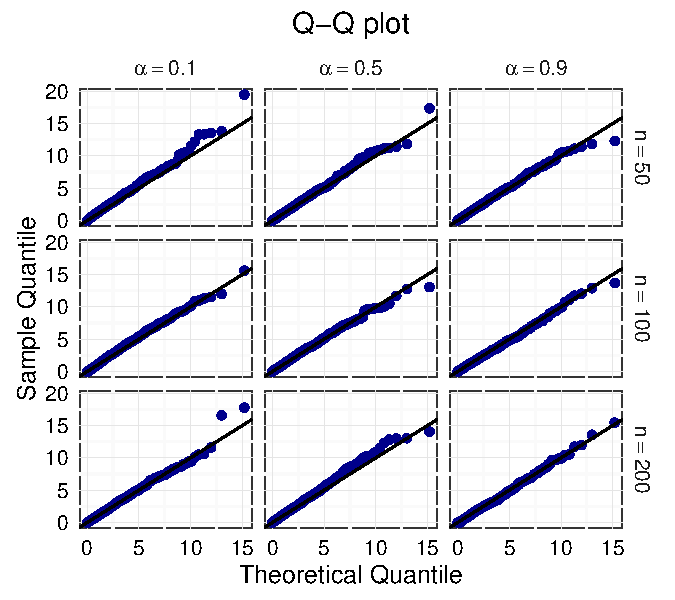
\includegraphics{myQQPlot.pdf}


We next consider another weight function $\pi (\theta; X)= N(\hat{\theta},\frac{1}{n}\hat{I}^{-1}_{\hat{\theta}})$. Lt $\hat{\theta}$ be the highest probability density estimator. And 
$$\hat{I}_\theta^{-1}=\sum_{i=1}^n
\begin{bmatrix}
-\frac{\partial^2 \log p_\theta(x_i)}{\partial \mu^2}&
    -\frac{\partial^2 \log p_\theta(x_i)}{\partial \mu\partial (\sigma^2)}
\\
    -\frac{\partial^2 \log p_\theta(x_i)}{\partial \mu\partial (\sigma^2)}
    &
    -\frac{\partial^2 \log p_\theta(x_i)}{\partial {(\sigma^2)}^2}
\end{bmatrix}$$
where

\begin{equation}
    \begin{aligned}
\frac{\partial^2 \log p_\theta(x)}{\partial
        \mu^2}=&
        \frac{(1-\alpha)({(x-\mu)}^2-1)dN(\mu,1)(x)+\alpha ({(x-\mu)}^2/\sigma^4 -\sigma^{-2})dN(\mu,\sigma^2)(x)}{p_\theta (x)}-\\
        &
        {\Big(\frac{(1-\alpha)(x-\mu)dN(\mu,1)(x)+\alpha(x-\mu)/\sigma^2 dN(\mu,\sigma^2)(x)}{p_\theta(x)}\Big)}^2,
    \end{aligned}
\end{equation}

\begin{equation}
    \begin{aligned}
        &\frac{\partial^2 \log p_\theta(x)}{\partial
        \mu\partial(\sigma^2)}=
        \frac{(\frac{3\alpha(\mu-x)}{2\sigma^4}-\frac{\alpha {(\mu-x)}^3}{2\sigma^6})dN(\mu,\sigma^2)(x)}{p_\theta (x)}-\\
        &
        \frac{\alpha (\frac{{(\mu-x)}^2}{2\sigma^4}-\frac{1}{2\sigma^2})dN(\mu,\sigma^2)(x)\big((1-\alpha)(x-\mu)dN(\mu,1)(x)+\alpha(x-\mu)/\sigma^2 d(\mu,\sigma^2)(x)\big)}{p_{\theta}{(x)}^2},
    \end{aligned}
\end{equation}


\begin{equation}
    \begin{aligned}
\frac{\partial^2 \log p_\theta(x)}{\partial
        {(\sigma^2)}^2}=&
        \frac{\alpha \big(\frac{3}{4\sigma^4}-\frac{3{(x-\mu)}^2}{2\sigma^6} +\frac{{(x-\mu)}^4}{4\sigma^8}\big)dN(\mu,\sigma^2)(x)}{p_\theta (x)}-\\
        &
        {\Big(\frac{\alpha\big(\frac{{(x-\mu)}^2}{2\sigma^4}-\frac{1}{2\sigma^2} \big)dN(\mu,\sigma^2)(x)}{p_\theta(x)}\Big)}^2.
    \end{aligned}
\end{equation}

We do the same simulation as above and the QQ-plot is given.
It  can be seen that the Wilks phenomenon still holds in this case.
For mixture model, sampling from posterior distribution is troublesome.
The computing burden will be reduce by normal approximation.
This is an advantage of normal weight ILRT.\@ From this example, we can see that ILRT is more flexible than posterior Bayes factor.


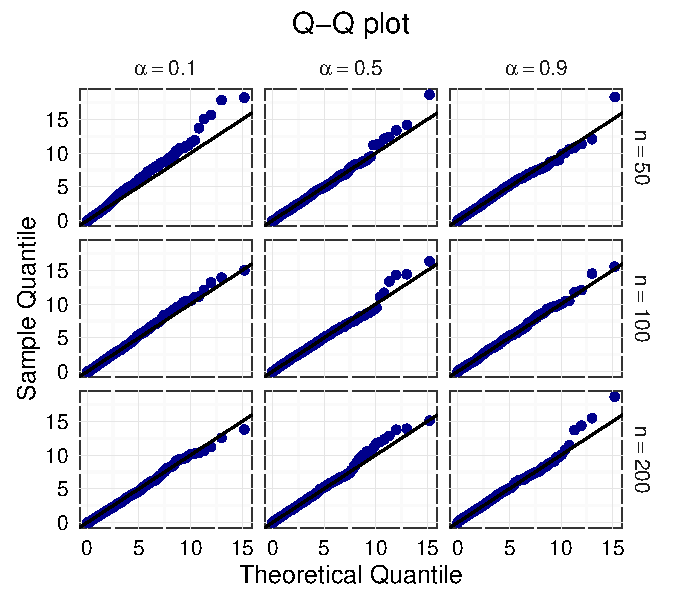
\includegraphics{myQQPlotNormal.pdf}





\section{Appendix}
For two measure sequence $P_n$ and $Q_n$ on measurable spaces $(\Omega_n,\mathcal{A}_n)$, denote by $P_n\triangleleft \triangleright Q_n$ that $P_n$ and $Q_n$ are mutually contiguous. That is, for any statistics $T_n$: $\Omega_n\mapsto \mathbb{R}^k$, we have $T_n\overset{P_n}{\rightsquigarrow}0\Leftrightarrow T_n\overset{Q_n}{\rightsquigarrow}0$.



\section*{References}

\bibliography{mybibfile}


\end{document}
